\chapter{Google App Engine.\label{ref_google_app_engine}}
En este apartado de la memoria voy a explicar lo que es, la configuración y el como usar la plataforma Google App Engine.

\section{Introduccion.\label{ref_introduccion_google_app_engine}}
Google App Engine es una conjunto de apis que proporciona Google para construir tus propias aplicaciones web, que pueden ser alojadas y usadas en su servicio Google App y vendidas en Google Apps Marketplace. Además de alojamiento gratuito Google, ofrecen un dominio, que es: \url{http://nombre\_de\_la\_aplicacion.appspot.com} y una base de datos propietaria de Google que se accede transparentemente a través de la api, gestión de usuarios mediante autentificación con cuentas Google del tipo: \textit{usuario@gmail.com}, autentificación por federación o \textit{openID}.

Además de todas esas características Google proporciona apis para Java, Python y Go, este último un lenguaje experimental del propio Google. Para usar dicha API, Google también da un plugin para Eclipse, en caso de que el lenguaje elegido sea Java, que ayuda al despliegue de la aplicación web, autocompletado y gestión de de las aplicaciones creadas. 
%TODO:En el anexo 1 se puede ver como instalar el puglins para eclipse de google app engine.

En el proyecto solo he usado la API de Google App Engine de Java, por lo que todo lo que puedo comentar es de dicha API, la parte de Python y Go no se han estudiado.

En general el uso de Google App Engine para crear aplicaciones web es idéntico a crear una aplicación web con Java 2 Enterprise Edition (Java2EE), se pueden crear servlet que recogen valores \textbf{GET} o \textbf{POST} y además clases java para hacer operaciones con dichos valores. A su vez para mostrar la infomación se pueden generar archivos \textit{*.jsp}, que son archivos html con bloques o líneas de código java que se introducen con estas etiquetas: $<$\%= línea de código Java \%$>$ o $<$\% Bloque de código Java \%$>$. A parte de archivos \textit{*.java} y \textit{*.jsp}, debemos tener una carpeta llamada \textit{war} en la que tiene que ir toda la información de la aplicación web que queremos deplegar. En dicha carpeta hay varias subcarpetas como pueden ser \textit{css} en la que tiene que ir el estilo de la web o \textit{WEB-INF} en la que están todos los archivos de configuración, como pueden ser los permisos que tenemos que tener para poder acceder al uso de un servlet, si la web tiene conexión https, la configuración de la base de datos, etc.

Para este proyecto se han tenido que desarrollar dos aplicaciones web, una que es un servidor de timestamp y otra que es una aplicación para gestión de las firmas digitales que realice cada usuario. A continuación vamos a explicar en profundida la tecnología usada y ambas aplicaciones web.

\section{Explicación de una aplicación web en Google App Engine.\label{ref_explicacion_google_app_engine}}
En esta parte voy a explicar en profundidad que es un servlet, los archivos de configuración, los archivos \textit{*.jsp} y el resto de archivos necesarios para poder desplegar una aplicación en Google Apps.
 
\subsection{¿Qué es un servlet?.}
Un servlet es la evolución de los antiguos applet, su uso más comun es generar páginas web dinámente con los parámetros que recibe mediante una petición realizada por el navegador web y datos que están almacenados en el servidor web.

Un servlet es un objeto java que tiene que ser ejecutado en un servidor web o contenedor J2EE, que recibe unos parámetros, realiza una o varias acciones y devuelve un resultado que puede ser desde un código html, un JSP que genera dinámicamente un código html, un JSON o una simple cadena de texto.

Los servlets, junto con JSP, son la solución de Oracle a la generación de contenido dinámico equivalente al lenguaje PHP, ASP de Microsoft, Ruby, etc.

Los servlet forman parte de Java Enterprise Edition (JEE) que a su vez es una amplicación de Java Standard Edition (JSE), para usarlos necesita un servidor web que pueda interpretar código java, el más famoso es Apache Tomcat que está desarrollado y mantenido por Apache Foundation, que son los encagardos también de mantener y desarrollar el famoso servidor web Apache, aunque existen otro como JBoss, Jetty o GlassFish, pero como veremos en este proyecto no son los únicos, ya que el propio Google Apps también funciona internamente a base de servlets y JSP.

Para crear un servlet hay que generar una clase java que implemente la interfaz \textit{javax.servlet.Servlet} o que extienda cualquier clase que herede de una clase o que implemente la interfaz anterior, como puede ser \textit{javax.servlet.http.HttpServlet} que es específico para conexiones HTTP. 
Una vez generada la clase hay que implementar el método \textbf{doGet} para peticiones tipo \textbf{GET} o el método \textbf{doPost} para peticiones de tipo \textbf{POST}. En el siguiente trozo se código se puede ver la implementación mas básica de los métodos \textbf{doGet} y \textbf{doPost}, con las llamadas sus respectivas llamadas a \textit{super}.

\begin{lstlisting}[language=Java] 

@Override
protected void doGet(HttpServletRequest req, 
	HttpServletResponse resp) throws ServletException, IOException {
	// TODO Auto-generated method stub
	super.doGet(req, resp);
}

@Override
protected void doPost(HttpServletRequest req, 
HttpServletResponse resp) throws ServletException, IOException {
	// TODO Auto-generated method stub
	super.doPost(req, resp);
}
\end{lstlisting}

Una vez implementados los métodos que se necesiten se pueden usar el parámetro \textit{HttpServletRequest req} para recibir los valores que queramos enviar a la aplicación web y podemos usar \textit{HttpServletResponse resp} para enviar lo que queramos desde una redirección a JSP o una página web a una JSON o cadena de texto. 
Un ejemplo de como se reciben los parámetros sería: 

\begin{lstlisting}[language=Java]  
String num_sec = req.getParameter("sec");
\end{lstlisting}

Y si queremos enviar algo por \textit{HttpServletResponse resp} podríamos usar:

\begin{lstlisting}[language=Java]   
PrintWriter out = resp.getWriter();
out.print(jsonArray);
out.flush();
\end{lstlisting}

Como podemos ver el objeto \textit{resp} nos da la posibilidad de conseguir un objeto \textit{java.io.PrintWriter} por el que podemos enviar lo que necesitemos.

%TODO: añadir la referencia... xD donde pone capítulo proximos xD
La forma de acceder a un servlet mandandole peticiones \textbf{GET} sería la siquiente: \url{https://servertimestamp.appspot.com/search?id=63&texto=Prueba}, como se puede ver la dirección base seria: \url{https://servertimestamp.appspot.com/}, el servlets estaría mapeado internamente en el servidor web, como ya veremos en próximas sección, en la dirección \url{/search} y el primer parámetro va precedido de \url{?id\_parámetro} y el resto de \url{\&id\_parámetro}. En nuestro ejemplo tendría dos parámetros que son \textit{id} y \textit{texto}, con sus respectivos valores después del =.

El método \textbf{POST} es el utilizado para pasar parámetros por medio de formularios.

\subsection{¿Qué es JSP?.\label{ref_jsp_google_app_engine}}
JSP es el acrónimo de JavaServer Pages y es una tecnología que ayuda a crear dinámicamente páginas web badas en HTML o XML y es la solución equivalente a PHP de Oracle. En la figura~\ref{fig:modoJSP} se puede observar el proceso que sigue desde que se hace la petición en el navegador hasta que se muestra.

\begin{figure}[hbt]
  \centering
    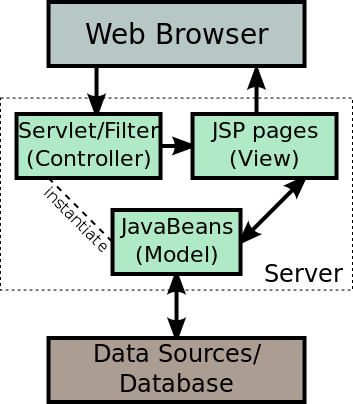
\includegraphics[scale=0.5]{./GoogleAppEngine/imagenes/JSP_Model.png}
  \caption{Modo de interpretación de un archivo JSP}
  \label{fig:modoJSP}
\end{figure}

Un fichero \textit{*.jsp} es la unión de código HTML con código java, el cual es interpretado en el momento de visualización de la página web. Un ejemplo es el siguiente:
 
\begin{lstlisting}[language=HTML]   
<!DOCTYPE html>
<html>
<body>
<table>
<tr>
	<th>ID</th>
	<th>Num sec</th>
	<th>Token de tiempo</th>
	<th>Mensaje</th>
	<th>URL para ver la firma</th>
	<th>Fecha</th>
	<th>Usuario</th>
	<th id="filadestino">Destino</th>
	<th>Verificado?</th>
</tr>

<% for (RowRepositorioGeneral row : rows) {%>
<tr>
	<td><%=row.getId()%></td>
	<td><%= row.getNum_sec()%></td>
	<td><%=row.getToken_tiempo()%></td>
	<td><%=row.getTexto_claro()%></td>
	<td><a href=<%=row.getUrl_firma()%>>URL para ver el token
			de tiempo</a></td>
	<td><%=row.getFecha()%></td>
	<td><%=row.getUsuario()%></td>
	<td id="filadestino"><%=row.getDestino()%></td>
	<td>
		<%
		Boolean confirmado = row.getConfirmado();
		if (!(confirmado == null) && confirmado) {
		%>
		<center>
			<img src="ok.png" />
		</center> <%} else  %>
	</td>
</tr>
<%}%>
</table>
</body>
</html>
\end{lstlisting}

Como se puede ver en este trozo de código este jsp genera una tabla que se rellena dinámicamente con los valores que devuelve un objeto java, se puede observar que se entrelazan trozos de código Java con etiquetas HTML. Si mostramos esta web y acto seguido introducimos otro objeto RowRepositorioGeneral en la estructura, cuando recarguemos la tabla tendrá una fila nueva.

\subsection{La carpeta WAR.}
La carpeta WAR es la carpeta principal para el despliegue de una aplicación web, ya que en ella es donde tienen que ir todos los archivos que necesitemos, desde archivos HTML, CSS, JSP, imágenes, etc. En la figura~\ref{fig:carpetawar} se puede ver un ejemplo de la carpeta WAR de mi aplicación web.

\begin{figure}[hbt]
  \centering
    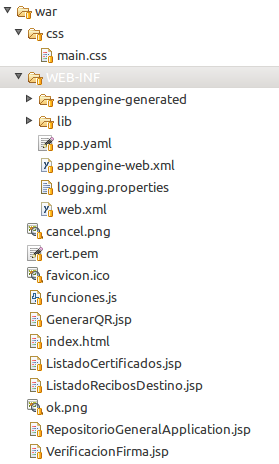
\includegraphics{./GoogleAppEngine/imagenes/carpetawar.png}
  \caption{Carpeta WAR}
  \label{fig:carpetawar}
\end{figure}

Se puede ver las diferentes carpetas y ficheros que la forman. Se ve la carpeta css que contiene los archivos de estilo que la página web usará, también se pueden ver los archivos \textit{web.xml} y \textit{app.yalm} que son archivos de configuración del servidor que se verán en el proximo apartado~\ref{ref_archivos_configuracion_google_app_engine} y además los archivos \textit{jsp} que se usan en la aplicación junto con los archivos \textit{html} y \textit{javascript} que se necesiten.

\subsection{Archivos de configuración.\label{ref_archivos_configuracion_google_app_engine}}
Los principales archivos de configuración son \textit{web.xml} y \textit{app.yalm}, este segundo es solo una forma de escribir de forma más legible el xml, para que nos sea más sencillo escribirlo y leerlo a los humanos.

Un ejemplo de un archivo \textit{web.xml} es el siguiente:

\begin{lstlisting}[language=XML]
<?xml version="1.0" encoding="utf-8"?>
<web-app xmlns:xsi="http://www.w3.org/2001/XMLSchema-instance"
xmlns="http://java.sun.com/xml/ns/javaee"
xmlns:web="http://java.sun.com/xml/ns/javaee/web-app_2_5.xsd"
xsi:schemaLocation="http://java.sun.com/xml/ns/javaee
http://java.sun.com/xml/ns/javaee/web-app_2_5.xsd" version="2.5">

	<servlet>
		<servlet-name>AddRow</servlet-name>
		<servlet-class>pfc.ServletCreateRow</servlet-class>
	</servlet>
	<servlet-mapping>
		<servlet-name>AddRow</servlet-name>
		<url-pattern>/add</url-pattern>
	</servlet-mapping>

	<welcome-file-list>
		<welcome-file>ServerTimestampApplication.jsp</welcome-file>
	</welcome-file-list>
</web-app>
\end{lstlisting}
%TODO: poner la referencia al código si se puede
Como se puede observar en el código se ha definido un servlet que se llamará \textbf{AddRow} que usará la clase \textbf{ServletCreateRow} y que estará mapeado en la dirección web \textbf{/add}, también podemos observar que el fichero que nos mostrará el servidor será \textbf{ServerTimestampApplication.jsp} si entramos a la url principal.

A continuación veremos como es un archivo \textit{app.yalm}:
\begin{lstlisting}[language=YAML]
application: repositoriorecibos
version: 1
runtime: java

handlers:
  - url: /add
    servlet: pfc.ServletCreateRow
    secure: always
welcome_files:
  - RepositorioGeneralApplication.jsp
\end{lstlisting}

Como podemos observar es mucho más fácil de entender y de escribir, el único problema que tienen los archivos YALM es que son sensibles a los espacios en blanco y tabuladores, por lo que hay que tener cuidado al redactarlos. En este archivo se crea un servlet en la ruta \textbf{/add}, que es la clase java \textbf{ServletCreateRow} del paquete \textbf{pfc} y que siempre hay que estar registrado en la aplicación para poder acceder a él. También podemos observar el fichero de bienvenida para cuando accedemos a la aplicación web. 
Al tener el archivo \textit{app.yalm} en la carpeta WEB-INF el parseador de YALM interpreta dicho archivo y genera un archivo \textit{web.xml} que es el que usará el servidor web para su configuración automáticamente.
\\
\\
Para ver todas las opciones de configuración que se pueden modificar en \textit{app.yalm} o en \textit{web.xml} se puede consultar estos enlaces \url{https://developers.google.com/appengine/docs/java/config/}, \url{https://developers.google.com/appengine/docs/java/configyaml/}. En el primero podemos ver todas las opciones configurables de \textit{web.xml} y el la segunda las de \textit{app.yalm}.
